\documentclass{article}
\usepackage{import}
\subimport{../}{preamble}
\begin{document}

\section{Plasmons in Tips}
\label{sec:tip_literature}

Significant efforts have been made to advance nanoscale surface characterisation by developing new optical tools and integrating optics into existing nanoscale topological measurements. Metallic tips were  investigated due to the widespread use of \glspl{spm}, such as \gls{afm}, and \gls{stm}. The similarity in size between metallic nanostructures and the sub-wavelength-size apex of tips initially suggested that visible plasmons would be expected, enabling resonant near-field enhancement. Prior to any spectral characterisation studies to understand their near-field response, tips were applied in combined SPM-optical microscopes to achieve sub-wavelength localisation and enhancement of optical signals. As the next logical step from \gls{sers} and \gls{snom}, the sharp apex of tips were exploited to develop the spin-off techniques of \gls{ters} \cite{stockle2000, anderson2000, hayazawa2000, pettinger2000} and \gls{asnom}%
\footnote{Also known as \gls{ssnom}.}
\cite{zenhausern1994, zenhausern1995, bachelot1995, knoll1997, knoll1998, keilmann1999}.
These are also known collectively as \gls{tenom}.%
\footnote{These are also sometimes known as field-enhancing near-field optical microscopy (FENOM) since apertured techniques do not necessarily exploit plasmonic enhancement as much.}

% TERS
The concept for TENOM was first proposed in 1985 \cite{wessel1985} but it was not until 2000 that reports first emerged using tips to enhance Raman spectroscopy \cite{stockle2000, anderson2000, hayazawa2000, pettinger2000}. All measurements were carried out in inverted microscopes with either an AFM \cite{stockle2000, anderson2000, hayazawa2000} or STM \cite{pettinger2000} mounted on top. Two of the initial measurements suggest the overall Raman enhancement has a lower limit of $\sim$\num{e4} \cite{stockle2000, anderson2000}, hence a field enhancement of around 10. A third independent measurement utilising evanescent wave excitation obtained an enhancement factor of 80 from a single tip apex, equivalent to the summed enhancement of many SERS hotspots on a Ag island film \cite{hayazawa2000}. Since then Raman enhancements in the region of \num{e7}--\num{e9} have been measured \cite{pettinger2012}.%
\footnote{A clear distinction is made between the field enhancement, $|E/E_0|$, and the Raman enhancement, $|E/E_0|^4$, when stating enhancement factors. In the literature the terms ``field enhancement" or ``enhancement factor" are generally used interchangeably between the magnitude of the near-field and the improvement in the Raman signal.}
Whilst SERS enhancement factors have also increased significantly in recent years, the TENOM approach remains popular since the tip can be scanned across a sample. For this reason, techniques such as TERS are widely considered to become the successors of SERS. However, for this to be the case, nanotips require the capability to controllably and reproducibly enhance the near-field. Understanding the electromagnetic response of metallised tips has therefore become of significant importance in recent years.
Since the use of tips for observing fundamental plasmonics is also a central part of this project it is beneficial to understand the underlying concepts and mechanisms of TENOM.

\begin{figure}[bt]
\begin{singlespace}
\centering
\begin{subfigure}[t]{0.47\textwidth}
	%\subimport{./figures/}{tenom_basic}
	\includegraphics{figures/tenom_basic}
\end{subfigure}
~
\begin{subfigure}[t]{0.47\textwidth}
	%\subimport{./figures/}{tenom_surface}
	\includegraphics{figures/tenom_surface}
\end{subfigure}
\end{singlespace}
\caption[Concepts of TENOM]{\textbf{Concepts of TENOM.} Basic TENOM systems constitute a tip and a sample (left). Tips can perturb evanescent surface waves, generated by high-NA TIR, and scatter them into the far-field ($1\rightarrow3$) \cite{neacsu2005, mehtani2006}. Photons illuminating the tip can induce a weak dipole localised to the tip apex, which can scatter the near-field ($2\rightarrow3$). More recent TENOM arrangements employ a metallic substrate to couple with the tip and further localise the field into a ``hot spot" (right). Coupling of plasmons between the tip and the substrate can be achieved by exciting SPPs on the substrate using evanescent waves (1) or by focusing light on the MIM gap such that the tip dipole induces an image dipole in the substrate (2). Both mechanisms lead to scattering of light from the gap into the far-field (3). SPPs launched onto the planar surface (either via the tip or evanescent waves) can radiatively decay into $\mathit{NA}>1$ ($1,2\rightarrow4$) \cite{wang2011}.}
\label{fig:tenom_concept}
\end{figure}

TENOM is ideally classified as a local excitation approach as opposed to a local scattering approach \cite{novotny2006}, though the two are not independent. \figurename~\ref{fig:tenom_concept} shows the general approaches to TENOM. In the tip scattering approach the non-radiative near-field, comprising evanescent waves, is perturbed by the presence of the tip, leading to scattering into radiative modes. In the tip excitation approach, the tip is resonantly excited to induce a large, local, near-field enhancement and used as a sub-diffraction-limited light source, from which  localised scattering can be measured. This process can be much more efficient than the pure scattering approach but depends on the optical antenna properties of the tip. In both cases, the resolution of scattering images is sub-diffraction limited and set by the size of the tip radius ($\sim$\SI{50}{nm}).

%\begin{figure}[bt]
%\centering
%\includegraphics[width=0.6\textwidth]{figures/literature/mauser2014a}
%\caption[Typical optical geometries found in TENOM experiments \cite{mauser2014}]{\textbf{Typical optical geometries found in TENOM experiments \cite{mauser2014}.} The most prominent system is the bottom-illumination/back-illumination configuration utilising high-NA objectives. The other main geometry is the side-illumination configuration.}
%\label{fig:ters_geometries}
%\end{figure}

To optimally exploit light scattering from nanoscopic tips, tip-based systems have been generally designed in either the side-illumination and bottom-illumination configuration (photon paths shown in \figurename~\ref{fig:tenom_concept}), setting the collection and, more importantly, the tip excitation geometry. Side-illumination has been used successfully in a number of cases \cite{mehtani2006, steidtner2007, zhang2013, wickramasinghe2014} but suffers generally from far-field scattering overshadowing the near-field. More complex optical techniques, such as using polarisation-resolved or interferometric approaches, are then required to overcome this. %In each case, side-illumination can be classified as a far-field excitation technique.
Bottom illumination, the more dominant design, utilises evanescent waves generated by $\NA>1$ illumination undergoing \gls{tir}. TIR results in minimal background scatter outside of the illumination aperture with only the near-field scatter collected. Collection is achieved using either the central $\NA<1$ aperture of the high \NA\ illumination objective \cite{hayazawa2001, yeo2006, yeo2007, zhang2013experimental, mino2014, kumar2014} or a secondary low NA objective \cite{hayazawa2007, taguchi2009, uetsuki2012}. Whilst this does require that both the sample and any metallic substrate are optically transmissive, evanescent wave generation can excite SPPs in both a metallic substrate and the tip once brought within the near-field. For these reasons, it is important to consider the optical geometry when interpreting any presented TENOM results.

\subsection{The Electromagnetic Response of Tips}

\begin{wrapfigure}{O}{0.45\textwidth}
\centering
\vspace{-15pt}
\includegraphics[width=\textwidth]{figures/lightning_rod_effect}
\vspace{-25pt}
\caption[Calculated magnitude of the electric field around a tip showing the lightning rod effect]{\textbf{Calculated magnitude of the electric field around a tip showing the lightning rod effect.} Compression of the field lines around the sharp corner of an equipotential surface leads to a localised, non-resonant field enhancement. Poisson's/Laplace's equation is solved for a tip structured electrode with a surface charge distribution separated by some distance from a planar metal counter electrode of the opposite surface charge.}
\label{fig:lightning_rod_effect}
\end{wrapfigure}

The electromagnetic response of tips can be broken down into individual components that constitute the enhancement mechanism. The two main optical components are the lightning rod effect and a resonant plasmon contribution for metallic tips \cite{esteban2006, zhang2009, schmid2013}. Each component is maximised when the incident field is along the tip axis \cite{zhang2014}. The plasmonic component has been the focus of study in recent tip-based work, however progress in sharpening tips has also led to increases in the lightning rod component. Both components are important to consider when attempting to understand optical measurements involving tips.

% The lightning rod effect in tips
Regardless of plasmonic behaviour, metallic tips intrinsically exhibit a lightning rod effect under the application of an applied field, instilling a non-resonant component of near-field enhancement. From the definition of the electric field $\vec{E}(\vec{r}) = -\nabla\pot(\vec{r})$ it is clear that the electric field strongly depends on geometry, with field lines perpendicular to the equipotential conductor surface. The more curved a surface, the more compressed the field lines become around its equipotential surface due to accumulation of surface charge.%
%This can be described by $E = \sigma/\epsfs$ where $\sigma = q/4\pi r^2$ is the surface charge density and $r$ is the radius of curvature.
\footnote{Since $E \propto 1/r^2$ the electric field is larger in regions of smaller curvature.}
A simple model, calculated by solving Laplace's equation for a tip-shaped electrode, shows this behaviour in \figurename~\ref{fig:lightning_rod_effect}. Consequently, even without a plasmonic component, sharp tips provide a promising platform for localised near-field enhancement.

% The plasmonic component
The expected plasmonic component also arises from the curvature of the metal-dielectric interface at the tip apex. Curvature allows for both SPP excitation and localisation at the apex due to adiabatic nanofocussing \cite{stockman2004, pile2006, berweger2010, lee2011, berweger2012, lindquist2013}. This can lead a number of localised plasmon modes in the predicted spectra of tips, however none of these will have an antenna-like geometry to couple well with far-field light. As highlighted when discussing ellipsoidal MNPs, strong, antenna-like LSPs are unlikely to be excited at the apex of a sharp tip since lack of a second metal-dielectric interface prevents accumulation of the opposite surface charge to the apex. Thus, there can be no strong restoring forces or \glspl{spr}. The extended size of the typical tip structure ($\sim$\SI{20}{\micro\metre}) prevents any potential low-order antenna-like plasmons from existing. Calculations for shorter tip geometries (nanocones or nanoellipsoids) show visible-NIR LSPs \cite{roth2006, goncharenko2006}, however these redshift and diminish with increasing tip length, leaving only the smooth response of the lightning rod effect increasing towards the IR \cite{zhang2009, huber2014}. The standard, sharp metallic tip geometry therefore makes for a poor \textit{plasmonic} optical antenna unless the optically-dark SPP modes can be accessed.

Evanescent waves are capable of exciting some of these modes, with evidence for localised apex plasmons found through resonant scattering of evanescent waves \cite{neacsu2005, mehtani2006, barrios2009}, resonances in the TERS background \cite{pettinger2007, pettinger2009} and depolarised scattering images \cite{mino2014}. The addition of a degree of nanostructuring also allows for more localised plasmons \cite{hayazawa2001, bailo2008, hayazawa2012, mino2014}.
Spectral resonances between 600--\SI{800}{nm} have been observed in scattered evanescent waves from the surface of a prism by a Au tip with W giving a comparatively flat spectrum \cite{neacsu2005}. These are attributed to SPPs. Shifts of $\sim$75--\SI{100}{nm} have been observed between Ag and Au tips with a Si\subs3N\subs4 underlying tip material, redshifting resonances by $\sim$\SI{30}{nm} compared with solid metallic tips \cite{mehtani2006, barrios2009}. This dependence on both the tip metal and underlying material has been highlighted numerous times due to the prevalence of the two dominant tip geometries of sharply etched metal tips and metallised (metal-coated) non-metallic tips.

\begin{figure}[bt]
\centering
\includegraphics[height=5cm, clip=true, trim=5 75 113 10]{figures/literature/nn-2014-031803_0002}
\includegraphics[height=5cm, clip=true, trim=170 180 140 280]{figures/literature/uetsuki2012supp}
%\includegraphics[width=0.3\textwidth, clip=true]{figures/literature/1-s2-0-S0009261401000653-gr1}
\includegraphics[height=5cm, clip=true, trim=20 5 0 165]{figures/literature/jrs4032-fig-0001}
\caption[]{\textbf{SEM images of metallised tips exhibiting random nanostructures.} Images are taken from \cite{mino2014} (left), \cite{uetsuki2012} (middle) and \cite{hayazawa2012} (right). Each SEM shows randomised grains deposited using evaporation. These are thought to enable LSP excitation if located at the apex.}
\label{fig:metallised_tips}
\end{figure}

Surface roughness imparted onto metallised tips by the coating procedure is likely to introduce localised plasmonic components which light can couple to, mimicking small 10--\SI{50}{nm} MNPs \cite{mino2014}. Similar behaviour has been used to explain the origin of SERS in rough metal films \cite{fleischmann1974, jeanmaire1977}. Each grain acts as a point at which photons couple and plasmons radiate, hence a grain located at the apex can plasmonically enhance and scatter the near-field. This behaviour is of importance in metallised dielectric tips coated using evaporation%
\footnote{Evaporation conditions used to roughly nanostructure a tip are similar to when depositing metal islands.}
\cite{hayazawa2001, hayazawa2012, mino2014} or chemical reactions \cite{bailo2008}, some examples of which are shown in \figurename~\ref{fig:metallised_tips}. Even with the frequent application of TENOM, there have been very few spectral measurements of scattering from tips from which to better understand tip plasmonics. Optimum tip parameters, such as coating thickness, for maximum field enhancement are still being debated and characterisation of performance is still carried out using TERS \cite{meng2015}.

% Theory work
%\cite{Demming2005, Rogov2013, behr2008}
Complete theoretical understanding of a tip's electromagnetic response is challenging due to difficulty in modelling tips. Their sub-wavelength apices and large ($\sim$\SI{20}{\micro\metre}) overall conical or pyramidal structure lead to complications when simulating their response, and approaches attempting to circumvent these limitations often cause physical inaccuracies in the result. Overly simplistic models, such as modelling only the tip apex, usually as a spherical or ellipsoidal MNP, fail to take into account the actual tip geometry, resulting in the existence of unphysical MNP-like modes at the tip apex. Similar multipolar modes are exhibited by truncated tip models with finite lengths less than \SI{1}{\micro\metre} \cite{roth2006, goncharenko2006}, behaving more like nanopyramids \cite{schafer2013, cherukulappurath2013}. Zhang \emph{et al.} \cite{zhang2009} calculate that between lengths of \SI{200}{nm} and infinity a tip transitions between supporting low order LSPs, then higher order LSPs, followed by only weak SPPs. LSPs are supported only when the entire tip structure is smaller in size than the focus, allowing light to drive in-phase collective oscillations of the conduction electrons. As the tip becomes larger, phase retardation occurs and higher order LSP modes dominate. Once the tip becomes larger than the focus, the case for almost all standard SPM tips, collective oscillations are no longer possible, leaving only weak LSPs concentrated at the apex and SPPs, whose periodic response in the field enhancement disappears with tip lengthening due to increased losses. Furthermore, the single metal-dielectric interface at the apex means that any LSPs similar to those in MNPs have much weaker dipole moments and are therefore much darker \cite{downes2006}. For realistic tip lengths all plasmon modes eventually disappear into a smooth, lightning rod continuum increasing into the IR \cite{zhang2009}.%
\footnote{The apparent sharpness of the apex increases with wavelength as the field becomes larger relative to the apex curvature. Thus the lightning rod effect is greater at longer wavelengths \cite{zhang2009}.}
As a result, smooth, sharp tips do not couple well with far-field light.

\subsubsection{Coupling with Metallic Substrates}

% Maybe work on that last paragraph
An alternative strategy is to couple tips with a planar metallic substrate and form a plasmonic \gls{mim} cavity to better localise light \cite{ren2004, neacsu2006, hayazawa2007, yano2007, pettinger2009, uetsuki2012, lindquist2013}. In this instance, a weakly-excited dipole in the tip can induce an image dipole in the metallic surface to form a more strongly-confined coupled mode in the gap. Specifically, pairing a Au tip with a Au substrate greatly enhances the field localisation and strength, moreso than when paired with a Pt surface \cite{ren2004} or a non-metallic surface \cite{downes2006}. This is attributed to better optical polarisability of the Au substrate. In these cases the Raman enhancement has been shown to rise to $\sim$\num{e7}--\num{e9} \cite{uetsuki2012}. Coupling can be achieved by either exciting the tip dipole or through SPP excitation on the underlying metallic substrate \cite{hayazawa2007, uetsuki2012}. Unlike the coupling between MNP plasmons, theory suggests that the coupling between a Au tip and a Au surface only minimally shifts the gap resonance \cite{downes2006}. % why?

% Electrical excitation
One final tip-based plasmon excitation mechanism of interest that has been discussed in recent years is electrical excitation. Similar to the use of \gls{eels} in electron microscopy, tunnelling electrons can be used to excite plasmons in an STM geometry. Since tips are typically illuminated with a single wavelength of light it becomes difficult to discern plasmonic features hidden in the collected light. Electrical excitation circumvents this limitation as electrons need only to have sufficient energy $eV$ that a portion transferred to the conduction electrons is enough to excite SPs with frequencies $\hbar\omega \leq eV$. Electrical excitation also functions to both remove background light contributions to spectra by removing the illumination source.

Using tunnelling current excitation, light has been observed from both the tip-air-metal substrate gap \cite{pettinger2007, pettinger2009} and the interface between the metal substrate and its underlying dielectric \cite{wang2011}. Broad resonances, which redshift with decreasing tip-sample separation, are found superimposed onto TERS spectra when operating in the STM configuration \cite{pettinger2007, pettinger2009}. These suggest the formation of a MIM gap mode. Light detected from metal-glass interfaces is leakage radiation from SPPs on the metal-air interface. Since light cannot leak from SPPs at the metal-air interface the detected light must be scattering from gap plasmons between the tip apex and the surface. It is thought that 95\% of the emission is due to SPP excitation rather than LSP excitation \cite{wang2011}.

\subsection{Challenges associated with Tip Plasmonics}

\begin{figure}
\centering
\fcapside[\FBwidth]
{\includegraphics[width=0.7\textwidth, clip=true, trim=0 35 0 0]{figures/literature/pc630379_f8}}
{\caption[Comparison of TERS field enhancements and contrasts reported between 2000 and 2011 \cite{pettinger2012}]{\textbf{Comparison of TERS field enhancements and contrasts reported between 2000 and 2011 \cite{pettinger2012}.} STM tips, likely due to their increased sharpness, outperform AFM tips. Ag tips outperform Au tips. Larger enhancements are observed in systems where there is an underlying thin, noble metallic film. Statistical correlations still remain somewhat weak, showing the current variability in TERS experiments, attributed to irreproducibility of enhancing tips.}
\label{fig:pettinger2012}}
\end{figure}

% Challenges for TERS and comparison between measurements
Since the initial measurements of tip enhancements and plasmons, techniques such as TERS and a-SNOM have become widespread. However, they are not currently reliable enough to be considered as a standard technique. Difficulty controlling the tip near-field is both a result of the irreproducibility of the tip geometry and a lack of understanding of the optical processes governing the enhancement, leading to large variations between reported field enhancements and TERS contrasts. A selection of these, reported between 2000 and 2011, are shown in \figurename~\ref{fig:pettinger2012}, showing the variability of TERS. The current challenges with TENOM are therefore improving the reproducibility of the near-field enhancement between tips \cite{blum2014, kumar2014, mino2014} and achieving a better understanding of the tips themselves \cite{zhang2009}.

% Sharpness and lightning rod effects
Factors determining the efficiency of TENOM include experimental excitation/collection geometry, tip sharpness, surface metal morphology, material influences and tip/apex orientation. From \figurename~\ref{fig:pettinger2012} it is clear that sharper STM tips result in larger field enhancements than metallised AFM tips and comparative studies have shown similar trends \cite{raschke2003, yeo2006, picardi2007}. Intuition suggests that the lightning rod effect must play a significant role in the near-field enhancement process. Theory showing drastic increases in the lightning rod effect after only small increases in sharpness (\SI{20}{nm} to \SI{10}{nm}) gives some evidence towards this \cite{zhang2009, meng2015}, potentially explaining the varying measured field enhancements over time and between experiments. However, sharpness-induced enhancements can only be improved to a point as recent theory indicates the existence of a quantum limit set by nonlocal effects \cite{wiener2012}.%
\footnote{Field enhancement saturates as the potential around any finer structural imperfections becomes smoothed due to electron spill-out (non-locality).}
Understanding how to optimise the plasmonic component in tips is therefore a priority.

% Material dependence
Materials choice, as with much of plasmonics, heavily influences any plasmonic behaviour. Ag tips generally outperform Au tips under visible light, although these claims highly depend on the underlying tip material and metal morphology. Only the metal and its morphology are important in solid STM tips and thickly metallised AFM tips, where plasmon energies are insensitive to any potential underlying materials. On thinly coated ($<\SI{40}{nm}$) AFM tips, plasmons are tuned by the metal film thickness \cite{huber2014} and the refractive index of the underlying tip material. Tuning can vary drastically between materials such as Si, SiO\subs2, and Si\subs3N\subs4 \cite{picardi2007, taguchi2009}. These high index materials can shift SPRs into the infrared and out of resonance with the pump laser frequency. Careful consideration must therefore be given when pairing a tip with a laser \cite{yeo2006, yeo2007, cui2007, hayazawa2012}.

% Morphology dependence
A large amount of variability stems from surface metal morphology. Reliance on randomised apex geometries, as shown in \figurename~\ref{fig:metallised_tips}, for LSP excitation greatly limits reproducibility. Furthermore, this granularity is rarely taken into theoretical account when attempting to mechanistically explain TENOM. The orientation of the tip, along with the roughened apex, with respect to the sample and the incident excitation field is also known to influence near-field enhancement \cite{yeo2006, mino2014}.

Finally, variability between similar measurements can stem simply from differences in tip placement, optical setup, whether coupled with a mirror, and the specific illumination/collection geometry or optics used. As tips are rarely characterised there is little traceability between measurements from which to systematically determine the relevant causes for difference. It is highly likely, however, that geometrical limitations are the current dominating limitation restricting the progress of TENOM, leading to research into new tip geometries with better optimised, well-known optical responses.

\subsection{Tip Modification, Nanostructuring and Optical Antenna Tips}

% Transitioning the discussion from sharp to nanostructured tips
The mode mismatch caused by the size difference between diffraction-limited light and the nanometre scale results in a 3--4 order of magnitude coupling efficiency loss \cite{berweger2010}. As described previously, a SP acts as an optical antenna. A good optical antenna has the ability to effectively modify the density of electromagnetic states such that the far-field radiation impedance is efficiently matched with the impedance of a near-field evanescent mode and vice versa \cite{novotny2006, novotny2011}. The antenna opens up scattering pathways between near-field emitters and the far-field by connecting wave states (\wvm-vectors) via new intermediate states (the plasmon). Evidence suggests that sharp metallic tips, in their standard form, are not particularly good optical antennae, with most modes unresponsive to far-field light. To improve their coupling efficiency, standard sharp tips have been modified or nanostructured to introduce the necessary intermediary plasmon states \cite{mauser2014}. Whilst previously achieved by roughening the metal surface, more reliable and reproducible methods have been developed in recent years to controllably nanostructure the tip and engineer the optical response.

% Grating tips as nanoscale light sources
Gratings imprinted onto the side of tips can transform the apex into a nanoscale, single wavelength light source as SPPs excited on the grating propagate to the apex and re-radiate on \SI{10}{nm} length scales \cite{neacsu2010}.%
\footnote{Single wavelength operation results from adiabatic nanofocussing of only a single $\lambda=\SI{800}{nm}$ mode.}
Far-field illumination remains spatially separated from the apex, suppressing background scatter and allowing only near-field scattering from the apex to be measured, producing background-free TERS signals \cite{berweger2010, berweger2012}.
% Nanoantennae tips
Nanostructuring of the tip apex has been investigated in order to engineer and tune an optical antenna precisely at the apex. Tips are structured with distinct, sub-wavelength-sized metallic features in order to create the necessary antenna-like LSPs to enable far-field excitation in the visible region of the EM spectrum. Etching \cite{uebel2013, kharintsev2013}, \gls{fib} machining \cite{weber2010, fleischer2011, maouli2015}, selective deposition \cite{zou2009}, MNP pickup \cite{denisyuk2012}, and nanostructure grafting \cite{huth2013} have all been successfully used to nanostructure optical antenna tips. Scattering resonances in the visible-NIR spectrum have been directly measured on a subset of these \cite{zou2009, maouli2015} while other reports use improvements in the field enhancement as a measurement of antenna quality \cite{umakoshi2012, huth2013, kharintsev2013}. In such cases the field enhancement can be improved by an order of magnitude through LSP excitation \cite{weber2010, fleischer2011, umakoshi2012}.

Lack of a strong plasmonic contribution from sharp Au metallised tips to TENOM is further evident from direct comparison with Au nanotip probes. A Si tip with the apex replaced by a Au nanocone outperforms a standard Au AFM tip by 120\% in the side illumination geometry \cite{huth2013}. Similarly, cutting the Au coating off past the apex also enables LSPs \cite{zou2009}. Each of these modifications is carried out using FIB machining and is therefore highly controllable, though costly in time and resources.
%{\color{red}Ideally, a simple geometry grafted onto the tip apex should be enough to open up the necessary plasmon states for far-field coupling.}

% Spherical nanostructuring
\begin{figure}[bt]
\centering
\begin{subfigure}[t]{0.35\textwidth}
	\includegraphics[width=\textwidth, clip=true, trim=0 0 0 130]{figures/literature/umakoshi2012a}
\end{subfigure}
~
\begin{subfigure}[t]{0.6\textwidth}
	\includegraphics[width=\textwidth, clip=true, trim=0 0 0 40]{figures/literature/nature11653-f1-2}
\end{subfigure}
\caption[Examples of spherical tip fabrication and surface plasmon resonances]{\textbf{Examples of spherical tip fabrication and surface plasmon resonances.} (left) Photochemically fabricated AgNP-on-Si tips for TERS \cite{umakoshi2012}. Field enhancement is increased $\sim$20$\times$ compared with sharp Ag tips when using \SI{488}{nm} illumination with a 1.4\,NA objective in an inverted microscope. (right) Experimental evidence of LSPs in \SI{50}{nm} Au-coated, \SI{150}{nm} radius spherical AFM probes (NanoTools B150) \cite{savage2012}. The large radius minimises sensitivity to axial tip-tip alignment, increases scattered signal levels, and supports higher-order plasmonic cavity modes in the visible spectrum. Resonances are far-field excited using a supercontinuum laser source in a side-illumination configuration. Separation-dependent coupling between two spherical tips confirms plasmonic behaviour.}
\label{fig:savage2012a}
\end{figure}

The simplest geometry to impart onto a tip apex is a sub-wavelength metal sphere. By doing so the tip gains LSPs similar to those in an isolated spherical MNP. The specific SPRs depend on the sphere material and geometry along with the attachment method since the base tip structure determines the local adjacent dielectric medium. Coupled SPRs between two spherical Au tips have been previously observed in the far-field \cite{savage2012}, but no characterisation has yet been done. Additionally, a 20$\times$ increase in field enhancement and spatial resolution has been measured when using a photochemically-fabricated AgNP-on-Si tip compared with a sharp Ag tip \cite{umakoshi2012}. These demonstrate that spherical metallic tips have the potential to improve TENOM if they can be fully understood.

To date there are very few reported methods of simply nanostructuring a tip without the need for FIB, electron microscopy or complex chemistry. A significant portion of the allocated project time was dedicated to determining a simple approach for chemically producing plasmonic tips, specifically targeting the spherical tip apex geometry. Other than their successful application in TERS and fundamental plasmonics studies, the origin of SPRs in spherical tips has not yet been fully investigated. Very little work has been done to reliably produce, characterise and understand the optics of spherically nanostructured tips. Furthermore, there is still work needed to similarly investigate the optical response of sharp tips, comparing them directly and quantitatively with nanostructured tips. Both types of tips can then be compared in both fundamental studies and near-field enhancement applications.

\end{document}